\documentclass{standalone}
\usepackage[latin1]{inputenc}
\usepackage{tikz}

\begin{document}
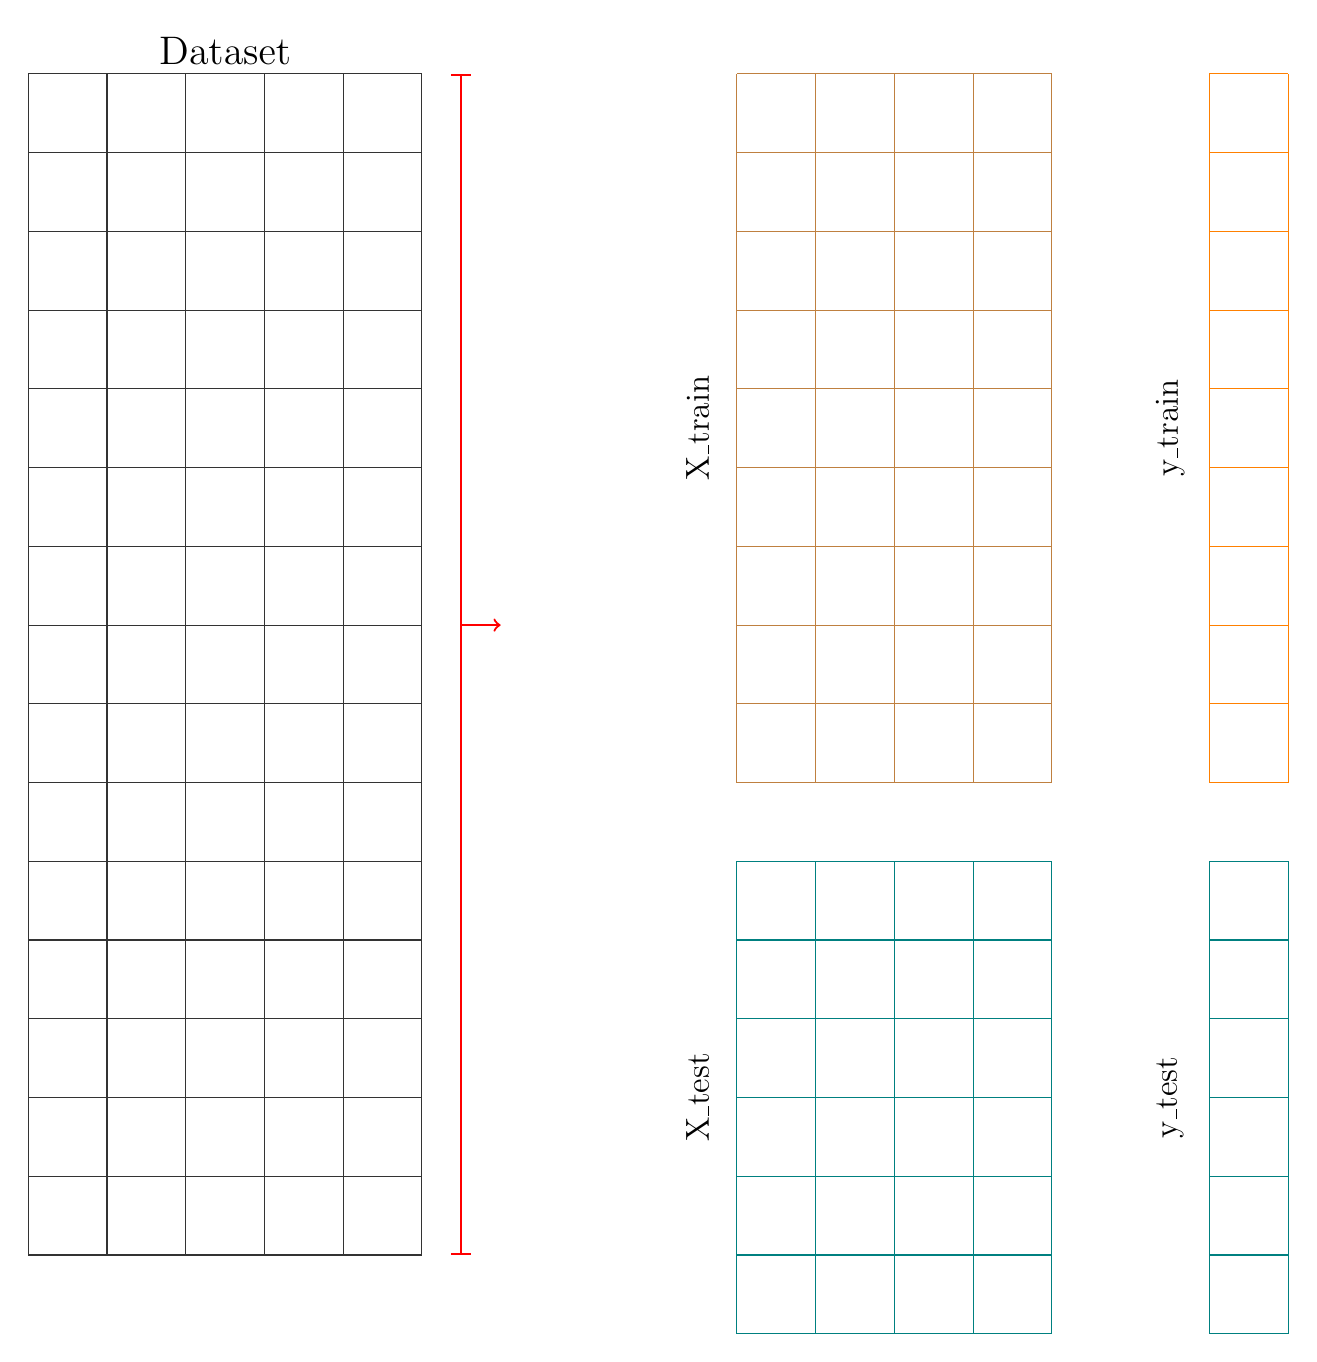
\begin{tikzpicture}
\draw[black!80] (0,0) grid (5,15);

\draw[brown] (9,6) grid (13,15);
\draw[orange] (15,6) grid (16,15);

\draw[teal] (9,-1) grid (13,5);
\draw[teal] (15,-1) grid (16,5);

\node[above] (a) at (2.5,15) {\Large Dataset};

\node[rotate=90] (a) at (8.5,10.5) {\large X\_train};
\node[rotate=90] (a) at (14.5,10.5) {\large y\_train};

\node[rotate=90] (a) at (8.5,2) {\large X\_test};
\node[rotate=90] (a) at (14.5,2) {\large y\_test};

\draw[->, red,thick] (5.5,8) -- (6,8);

\draw[|-|, red,thick] (5.5,0) -- (5.5,15);
\end{tikzpicture}

\end{document}